\documentclass[1p]{elsarticle_modified}
%\bibliographystyle{elsarticle-num}

%\usepackage[colorlinks]{hyperref}
%\usepackage{abbrmath_seonhwa} %\Abb, \Ascr, \Acal ,\Abf, \Afrak
\usepackage{amsfonts}
\usepackage{amssymb}
\usepackage{amsmath}
\usepackage{amsthm}
\usepackage{scalefnt}
\usepackage{amsbsy}
\usepackage{kotex}
\usepackage{caption}
\usepackage{subfig}
\usepackage{color}
\usepackage{graphicx}
\usepackage{xcolor} %% white, black, red, green, blue, cyan, magenta, yellow
\usepackage{float}
\usepackage{setspace}
\usepackage{hyperref}

\usepackage{tikz}
\usetikzlibrary{arrows}

\usepackage{multirow}
\usepackage{array} % fixed length table
\usepackage{hhline}

%%%%%%%%%%%%%%%%%%%%%
\makeatletter
\renewcommand*\env@matrix[1][\arraystretch]{%
	\edef\arraystretch{#1}%
	\hskip -\arraycolsep
	\let\@ifnextchar\new@ifnextchar
	\array{*\c@MaxMatrixCols c}}
\makeatother %https://tex.stackexchange.com/questions/14071/how-can-i-increase-the-line-spacing-in-a-matrix
%%%%%%%%%%%%%%%

\usepackage[normalem]{ulem}

\newcommand{\msout}[1]{\ifmmode\text{\sout{\ensuremath{#1}}}\else\sout{#1}\fi}
%SOURCE: \msout is \stkout macro in https://tex.stackexchange.com/questions/20609/strikeout-in-math-mode

\newcommand{\cancel}[1]{
	\ifmmode
	{\color{red}\msout{#1}}
	\else
	{\color{red}\sout{#1}}
	\fi
}

\newcommand{\add}[1]{
	{\color{blue}\uwave{#1}}
}

\newcommand{\replace}[2]{
	\ifmmode
	{\color{red}\msout{#1}}{\color{blue}\uwave{#2}}
	\else
	{\color{red}\sout{#1}}{\color{blue}\uwave{#2}}
	\fi
}

\newcommand{\Sol}{\mathcal{S}} %segment
\newcommand{\D}{D} %diagram
\newcommand{\A}{\mathcal{A}} %arc


%%%%%%%%%%%%%%%%%%%%%%%%%%%%%5 test

\def\sl{\operatorname{\textup{SL}}(2,\Cbb)}
\def\psl{\operatorname{\textup{PSL}}(2,\Cbb)}
\def\quan{\mkern 1mu \triangleright \mkern 1mu}

\theoremstyle{definition}
\newtheorem{thm}{Theorem}[section]
\newtheorem{prop}[thm]{Proposition}
\newtheorem{lem}[thm]{Lemma}
\newtheorem{ques}[thm]{Question}
\newtheorem{cor}[thm]{Corollary}
\newtheorem{defn}[thm]{Definition}
\newtheorem{exam}[thm]{Example}
\newtheorem{rmk}[thm]{Remark}
\newtheorem{alg}[thm]{Algorithm}

\newcommand{\I}{\sqrt{-1}}
\begin{document}

%\begin{frontmatter}
%
%\title{Boundary parabolic representations of knots up to 8 crossings}
%
%%% Group authors per affiliation:
%\author{Yunhi Cho} 
%\address{Department of Mathematics, University of Seoul, Seoul, Korea}
%\ead{yhcho@uos.ac.kr}
%
%
%\author{Seonhwa Kim} %\fnref{s_kim}}
%\address{Center for Geometry and Physics, Institute for Basic Science, Pohang, 37673, Korea}
%\ead{ryeona17@ibs.re.kr}
%
%\author{Hyuk Kim}
%\address{Department of Mathematical Sciences, Seoul National University, Seoul 08826, Korea}
%\ead{hyukkim@snu.ac.kr}
%
%\author{Seokbeom Yoon}
%\address{Department of Mathematical Sciences, Seoul National University, Seoul, 08826,  Korea}
%\ead{sbyoon15@snu.ac.kr}
%
%\begin{abstract}
%We find all boundary parabolic representation of knots up to 8 crossings.
%
%\end{abstract}
%\begin{keyword}
%    \MSC[2010] 57M25 
%\end{keyword}
%
%\end{frontmatter}

%\linenumbers
%\tableofcontents
%
\newcommand\colored[1]{\textcolor{white}{\rule[-0.35ex]{0.8em}{1.4ex}}\kern-0.8em\color{red} #1}%
%\newcommand\colored[1]{\textcolor{white}{ #1}\kern-2.17ex	\textcolor{white}{ #1}\kern-1.81ex	\textcolor{white}{ #1}\kern-2.15ex\color{red}#1	}

{\Large $\underline{11a_{127}~(K11a_{127})}$}

\setlength{\tabcolsep}{10pt}
\renewcommand{\arraystretch}{1.6}
\vspace{1cm}\begin{tabular}{m{100pt}>{\centering\arraybackslash}m{274pt}}
\multirow{5}{120pt}{
	\centering
	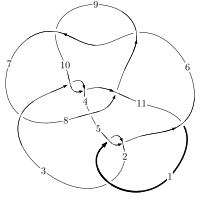
\includegraphics[width=112pt]{../../../GIT/diagram.site/Diagrams/png/376_11a_127.png}\\
\ \ \ A knot diagram\footnotemark}&
\allowdisplaybreaks
\textbf{Linearized knot diagam} \\
\cline{2-2}
 &
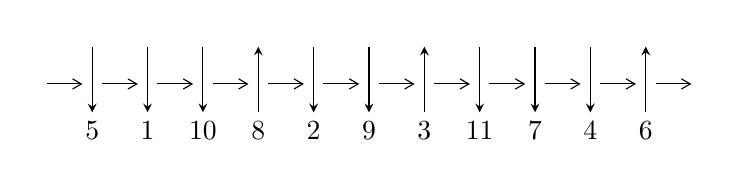
\begin{tikzpicture}[x=20pt, y=17pt]
	% nodes
	\node (C0) at (0, 0) {};
	\node (C1) at (1, 0) {};
	\node (C1U) at (1, +1) {};
	\node (C1D) at (1, -1) {5};

	\node (C2) at (2, 0) {};
	\node (C2U) at (2, +1) {};
	\node (C2D) at (2, -1) {1};

	\node (C3) at (3, 0) {};
	\node (C3U) at (3, +1) {};
	\node (C3D) at (3, -1) {10};

	\node (C4) at (4, 0) {};
	\node (C4U) at (4, +1) {};
	\node (C4D) at (4, -1) {8};

	\node (C5) at (5, 0) {};
	\node (C5U) at (5, +1) {};
	\node (C5D) at (5, -1) {2};

	\node (C6) at (6, 0) {};
	\node (C6U) at (6, +1) {};
	\node (C6D) at (6, -1) {9};

	\node (C7) at (7, 0) {};
	\node (C7U) at (7, +1) {};
	\node (C7D) at (7, -1) {3};

	\node (C8) at (8, 0) {};
	\node (C8U) at (8, +1) {};
	\node (C8D) at (8, -1) {11};

	\node (C9) at (9, 0) {};
	\node (C9U) at (9, +1) {};
	\node (C9D) at (9, -1) {7};

	\node (C10) at (10, 0) {};
	\node (C10U) at (10, +1) {};
	\node (C10D) at (10, -1) {4};

	\node (C11) at (11, 0) {};
	\node (C11U) at (11, +1) {};
	\node (C11D) at (11, -1) {6};
	\node (C12) at (12, 0) {};

	% arrows
	\draw[->,>={angle 60}]
	(C0) edge (C1) (C1) edge (C2) (C2) edge (C3) (C3) edge (C4) (C4) edge (C5) (C5) edge (C6) (C6) edge (C7) (C7) edge (C8) (C8) edge (C9) (C9) edge (C10) (C10) edge (C11) (C11) edge (C12) ;	\draw[->,>=stealth]
	(C1U) edge (C1D) (C2U) edge (C2D) (C3U) edge (C3D) (C4D) edge (C4U) (C5U) edge (C5D) (C6U) edge (C6D) (C7D) edge (C7U) (C8U) edge (C8D) (C9U) edge (C9D) (C10U) edge (C10D) (C11D) edge (C11U) ;
	\end{tikzpicture} \\
\hhline{~~} \\& 
\textbf{Solving Sequence} \\ \cline{2-2} 
 &
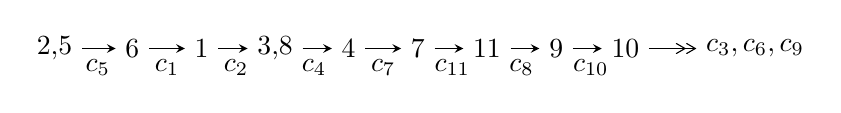
\begin{tikzpicture}[x=25pt, y=7pt]
	% node
	\node (A0) at (-1/8, 0) {2,5};
	\node (A1) at (1, 0) {6};
	\node (A2) at (2, 0) {1};
	\node (A3) at (49/16, 0) {3,8};
	\node (A4) at (33/8, 0) {4};
	\node (A5) at (41/8, 0) {7};
	\node (A6) at (49/8, 0) {11};
	\node (A7) at (57/8, 0) {9};
	\node (A8) at (65/8, 0) {10};
	\node (C1) at (1/2, -1) {$c_{5}$};
	\node (C2) at (3/2, -1) {$c_{1}$};
	\node (C3) at (5/2, -1) {$c_{2}$};
	\node (C4) at (29/8, -1) {$c_{4}$};
	\node (C5) at (37/8, -1) {$c_{7}$};
	\node (C6) at (45/8, -1) {$c_{11}$};
	\node (C7) at (53/8, -1) {$c_{8}$};
	\node (C8) at (61/8, -1) {$c_{10}$};
	\node (A9) at (10, 0) {$c_{3},c_{6},c_{9}$};

	% edge
	\draw[->,>=stealth]	
	(A0) edge (A1) (A1) edge (A2) (A2) edge (A3) (A3) edge (A4) (A4) edge (A5) (A5) edge (A6) (A6) edge (A7) (A7) edge (A8) ;
	\draw[->>,>={angle 60}]	
	(A8) edge (A9);
\end{tikzpicture} \\ 

\end{tabular} \\

\footnotetext{
The image of knot diagram is generated by the software ``\textbf{Draw programme}" developed by Andrew Bartholomew(\url{http://www.layer8.co.uk/maths/draw/index.htm\#Running-draw}), where we modified some parts for our purpose(\url{https://github.com/CATsTAILs/LinksPainter}).
}\phantom \\ \newline 
\centering \textbf{Ideals for irreducible components\footnotemark of $X_{\text{par}}$} 
 
\begin{align*}
I^u_{1}&=\langle 
-1.48129\times10^{37} u^{70}-2.24416\times10^{37} u^{69}+\cdots+2.11503\times10^{37} b+2.31427\times10^{37},\\
\phantom{I^u_{1}}&\phantom{= \langle  }1.02558\times10^{37} u^{70}+1.31834\times10^{37} u^{69}+\cdots+9.61375\times10^{36} a-1.17173\times10^{37},\;u^{71}+2 u^{70}+\cdots-2 u-1\rangle \\
I^u_{2}&=\langle 
b,\;3 u^2+5 a-7 u+6,\;u^3- u^2+1\rangle \\
\\
\end{align*}
\raggedright * 2 irreducible components of $\dim_{\mathbb{C}}=0$, with total 74 representations.\\
\footnotetext{All coefficients of polynomials are rational numbers. But the coefficients are sometimes approximated in decimal forms when there is not enough margin.}
\newpage
\renewcommand{\arraystretch}{1}
\centering \section*{I. $I^u_{1}= \langle -1.48\times10^{37} u^{70}-2.24\times10^{37} u^{69}+\cdots+2.12\times10^{37} b+2.31\times10^{37},\;1.03\times10^{37} u^{70}+1.32\times10^{37} u^{69}+\cdots+9.61\times10^{36} a-1.17\times10^{37},\;u^{71}+2 u^{70}+\cdots-2 u-1 \rangle$}
\flushleft \textbf{(i) Arc colorings}\\
\begin{tabular}{m{7pt} m{180pt} m{7pt} m{180pt} }
\flushright $a_{2}=$&$\begin{pmatrix}0\\u\end{pmatrix}$ \\
\flushright $a_{5}=$&$\begin{pmatrix}1\\0\end{pmatrix}$ \\
\flushright $a_{6}=$&$\begin{pmatrix}1\\u^2\end{pmatrix}$ \\
\flushright $a_{1}=$&$\begin{pmatrix}u\\u\end{pmatrix}$ \\
\flushright $a_{3}=$&$\begin{pmatrix}- u^3\\- u^3+u\end{pmatrix}$ \\
\flushright $a_{8}=$&$\begin{pmatrix}-1.06678 u^{70}-1.37130 u^{69}+\cdots+3.23612 u+1.21881\\0.700363 u^{70}+1.06106 u^{69}+\cdots-0.692179 u-1.09420\end{pmatrix}$ \\
\flushright $a_{4}=$&$\begin{pmatrix}-2.15925 u^{70}-2.76790 u^{69}+\cdots+1.95352 u+2.23161\\-0.0889259 u^{70}-0.0397494 u^{69}+\cdots+0.558128 u-0.272953\end{pmatrix}$ \\
\flushright $a_{7}=$&$\begin{pmatrix}-0.0510485 u^{70}-0.373547 u^{69}+\cdots+2.27625 u+0.706786\\1.65193 u^{70}+2.44250 u^{69}+\cdots-2.69769 u-2.53117\end{pmatrix}$ \\
\flushright $a_{11}=$&$\begin{pmatrix}u^3\\u^5- u^3+u\end{pmatrix}$ \\
\flushright $a_{9}=$&$\begin{pmatrix}-1.48850 u^{70}-2.21759 u^{69}+\cdots+3.68765 u+1.74401\\0.992194 u^{70}+1.60425 u^{69}+\cdots-2.38134 u-1.45862\end{pmatrix}$ \\
\flushright $a_{10}=$&$\begin{pmatrix}2.15925 u^{70}+2.76790 u^{69}+\cdots-1.95352 u-2.23161\\1.20977 u^{70}+1.41960 u^{69}+\cdots-0.383830 u-1.82356\end{pmatrix}$\\ \flushright $a_{10}=$&$\begin{pmatrix}2.15925 u^{70}+2.76790 u^{69}+\cdots-1.95352 u-2.23161\\1.20977 u^{70}+1.41960 u^{69}+\cdots-0.383830 u-1.82356\end{pmatrix}$\\&\end{tabular}
\flushleft \textbf{(ii) Obstruction class $= -1$}\\~\\
\flushleft \textbf{(iii) Cusp Shapes $= 0.637188 u^{70}+2.00147 u^{69}+\cdots+4.31419 u-9.38239$}\\~\\
\newpage\renewcommand{\arraystretch}{1}
\flushleft \textbf{(iv) u-Polynomials at the component}\newline \\
\begin{tabular}{m{50pt}|m{274pt}}
Crossings & \hspace{64pt}u-Polynomials at each crossing \\
\hline $$\begin{aligned}c_{1},c_{5}\end{aligned}$$&$\begin{aligned}
&u^{71}+2 u^{70}+\cdots-2 u-1
\end{aligned}$\\
\hline $$\begin{aligned}c_{2}\end{aligned}$$&$\begin{aligned}
&u^{71}+36 u^{70}+\cdots+4 u+1
\end{aligned}$\\
\hline $$\begin{aligned}c_{3},c_{10}\end{aligned}$$&$\begin{aligned}
&u^{71}+2 u^{70}+\cdots-4 u-1
\end{aligned}$\\
\hline $$\begin{aligned}c_{4}\end{aligned}$$&$\begin{aligned}
&u^{71}-3 u^{70}+\cdots+660 u+200
\end{aligned}$\\
\hline $$\begin{aligned}c_{6},c_{9}\end{aligned}$$&$\begin{aligned}
&u^{71}-4 u^{70}+\cdots+21 u-25
\end{aligned}$\\
\hline $$\begin{aligned}c_{7}\end{aligned}$$&$\begin{aligned}
&5(5 u^{71}-39 u^{70}+\cdots+379583 u+94103)
\end{aligned}$\\
\hline $$\begin{aligned}c_{8}\end{aligned}$$&$\begin{aligned}
&5(5 u^{71}-6 u^{70}+\cdots+231980 u-42881)
\end{aligned}$\\
\hline $$\begin{aligned}c_{11}\end{aligned}$$&$\begin{aligned}
&u^{71}+6 u^{70}+\cdots-6402 u-847
\end{aligned}$\\
\hline
\end{tabular}\\~\\
\newpage\renewcommand{\arraystretch}{1}
\flushleft \textbf{(v) Riley Polynomials at the component}\newline \\
\begin{tabular}{m{50pt}|m{274pt}}
Crossings & \hspace{64pt}Riley Polynomials at each crossing \\
\hline $$\begin{aligned}c_{1},c_{5}\end{aligned}$$&$\begin{aligned}
&y^{71}-36 y^{70}+\cdots+4 y-1
\end{aligned}$\\
\hline $$\begin{aligned}c_{2}\end{aligned}$$&$\begin{aligned}
&y^{71}+72 y^{69}+\cdots+16 y-1
\end{aligned}$\\
\hline $$\begin{aligned}c_{3},c_{10}\end{aligned}$$&$\begin{aligned}
&y^{71}-48 y^{70}+\cdots+4 y-1
\end{aligned}$\\
\hline $$\begin{aligned}c_{4}\end{aligned}$$&$\begin{aligned}
&y^{71}+21 y^{70}+\cdots-606000 y-40000
\end{aligned}$\\
\hline $$\begin{aligned}c_{6},c_{9}\end{aligned}$$&$\begin{aligned}
&y^{71}-58 y^{70}+\cdots+79841 y-625
\end{aligned}$\\
\hline $$\begin{aligned}c_{7}\end{aligned}$$&$\begin{aligned}
&25(25 y^{71}+959 y^{70}+\cdots-1.81656\times10^{11} y-8.85537\times10^{9})
\end{aligned}$\\
\hline $$\begin{aligned}c_{8}\end{aligned}$$&$\begin{aligned}
&25(25 y^{71}-936 y^{70}+\cdots+3.67278\times10^{10} y-1.83878\times10^{9})
\end{aligned}$\\
\hline $$\begin{aligned}c_{11}\end{aligned}$$&$\begin{aligned}
&y^{71}+36 y^{70}+\cdots+22222860 y-717409
\end{aligned}$\\
\hline
\end{tabular}\\~\\
\newpage\flushleft \textbf{(vi) Complex Volumes and Cusp Shapes}
$$\begin{array}{c|c|c}  
\text{Solutions to }I^u_{1}& \I (\text{vol} + \sqrt{-1}CS) & \text{Cusp shape}\\
 \hline 
\begin{aligned}
u &= -0.756248 + 0.731356 I \\
a &= -0.319350 - 0.556979 I \\
b &= -0.609727 + 0.867860 I\end{aligned}
 & -4.07719 - 3.90151 I & -5.00000 + 3.54699 I \\ \hline\begin{aligned}
u &= -0.756248 - 0.731356 I \\
a &= -0.319350 + 0.556979 I \\
b &= -0.609727 - 0.867860 I\end{aligned}
 & -4.07719 + 3.90151 I & -5.00000 - 3.54699 I \\ \hline\begin{aligned}
u &= -0.815711 + 0.480281 I \\
a &= \phantom{-}0.851857 + 0.985100 I \\
b &= \phantom{-}0.795395 - 0.523783 I\end{aligned}
 & -0.567421 - 0.429034 I & -3.85529 - 0.87645 I \\ \hline\begin{aligned}
u &= -0.815711 - 0.480281 I \\
a &= \phantom{-}0.851857 - 0.985100 I \\
b &= \phantom{-}0.795395 + 0.523783 I\end{aligned}
 & -0.567421 + 0.429034 I & -3.85529 + 0.87645 I \\ \hline\begin{aligned}
u &= -0.270630 + 0.894068 I \\
a &= -0.243231 + 0.020060 I \\
b &= -0.051628 - 0.966961 I\end{aligned}
 & -7.01345 + 0.86966 I & -12.36097 - 1.34990 I \\ \hline\begin{aligned}
u &= -0.270630 - 0.894068 I \\
a &= -0.243231 - 0.020060 I \\
b &= -0.051628 + 0.966961 I\end{aligned}
 & -7.01345 - 0.86966 I & -12.36097 + 1.34990 I \\ \hline\begin{aligned}
u &= \phantom{-}0.916597 + 0.577342 I \\
a &= \phantom{-}0.034897 - 0.799407 I \\
b &= \phantom{-}0.811438 + 0.019369 I\end{aligned}
 & \phantom{-}1.66910 - 3.91281 I & \phantom{-0.000000 } 0 \\ \hline\begin{aligned}
u &= \phantom{-}0.916597 - 0.577342 I \\
a &= \phantom{-}0.034897 + 0.799407 I \\
b &= \phantom{-}0.811438 - 0.019369 I\end{aligned}
 & \phantom{-}1.66910 + 3.91281 I & \phantom{-0.000000 } 0 \\ \hline\begin{aligned}
u &= -0.836576 + 0.691781 I \\
a &= -0.894496 + 0.459599 I \\
b &= \phantom{-}0.799336 + 0.956428 I\end{aligned}
 & -4.32946 + 9.25395 I & \phantom{-0.000000 } 0 \\ \hline\begin{aligned}
u &= -0.836576 - 0.691781 I \\
a &= -0.894496 - 0.459599 I \\
b &= \phantom{-}0.799336 - 0.956428 I\end{aligned}
 & -4.32946 - 9.25395 I & \phantom{-0.000000 } 0\\
 \hline 
 \end{array}$$\newpage$$\begin{array}{c|c|c}  
\text{Solutions to }I^u_{1}& \I (\text{vol} + \sqrt{-1}CS) & \text{Cusp shape}\\
 \hline 
\begin{aligned}
u &= \phantom{-}0.222287 + 0.874807 I \\
a &= -0.288795 + 0.326260 I \\
b &= \phantom{-}0.664290 + 0.919235 I\end{aligned}
 & -2.91874 + 5.72330 I & -6.82100 - 5.17076 I \\ \hline\begin{aligned}
u &= \phantom{-}0.222287 - 0.874807 I \\
a &= -0.288795 - 0.326260 I \\
b &= \phantom{-}0.664290 - 0.919235 I\end{aligned}
 & -2.91874 - 5.72330 I & -6.82100 + 5.17076 I \\ \hline\begin{aligned}
u &= -0.730824 + 0.527079 I \\
a &= \phantom{-}0.753832 - 0.354136 I \\
b &= -0.968868 - 0.896754 I\end{aligned}
 & -0.33023 + 4.59723 I & -4.06867 - 6.98717 I \\ \hline\begin{aligned}
u &= -0.730824 - 0.527079 I \\
a &= \phantom{-}0.753832 + 0.354136 I \\
b &= -0.968868 + 0.896754 I\end{aligned}
 & -0.33023 - 4.59723 I & -4.06867 + 6.98717 I \\ \hline\begin{aligned}
u &= \phantom{-}0.852440 + 0.278118 I \\
a &= -0.491553 + 0.803598 I \\
b &= \phantom{-}0.441660 + 1.237110 I\end{aligned}
 & -4.80199 - 3.21094 I & -12.45295 + 5.85076 I \\ \hline\begin{aligned}
u &= \phantom{-}0.852440 - 0.278118 I \\
a &= -0.491553 - 0.803598 I \\
b &= \phantom{-}0.441660 - 1.237110 I\end{aligned}
 & -4.80199 + 3.21094 I & -12.45295 - 5.85076 I \\ \hline\begin{aligned}
u &= -0.234589 + 0.853865 I \\
a &= -0.554053 - 0.463968 I \\
b &= \phantom{-}1.02317 - 1.27672 I\end{aligned}
 & -7.77113 - 11.46490 I & -8.41846 + 5.96289 I \\ \hline\begin{aligned}
u &= -0.234589 - 0.853865 I \\
a &= -0.554053 + 0.463968 I \\
b &= \phantom{-}1.02317 + 1.27672 I\end{aligned}
 & -7.77113 + 11.46490 I & -8.41846 - 5.96289 I \\ \hline\begin{aligned}
u &= \phantom{-}0.640616 + 0.584471 I \\
a &= \phantom{-}0.569021 + 0.397714 I \\
b &= -0.836952 + 0.262697 I\end{aligned}
 & \phantom{-}2.46408 - 0.68931 I & \phantom{-}1.74747 + 0.77475 I \\ \hline\begin{aligned}
u &= \phantom{-}0.640616 - 0.584471 I \\
a &= \phantom{-}0.569021 - 0.397714 I \\
b &= -0.836952 - 0.262697 I\end{aligned}
 & \phantom{-}2.46408 + 0.68931 I & \phantom{-}1.74747 - 0.77475 I\\
 \hline 
 \end{array}$$\newpage$$\begin{array}{c|c|c}  
\text{Solutions to }I^u_{1}& \I (\text{vol} + \sqrt{-1}CS) & \text{Cusp shape}\\
 \hline 
\begin{aligned}
u &= -0.859660\phantom{ +0.000000I} \\
a &= -0.477948\phantom{ +0.000000I} \\
b &= \phantom{-}1.49255\phantom{ +0.000000I}\end{aligned}
 & -6.41668\phantom{ +0.000000I} & -15.8580\phantom{ +0.000000I} \\ \hline\begin{aligned}
u &= -1.099450 + 0.364554 I \\
a &= \phantom{-}0.87164 - 1.32285 I \\
b &= \phantom{-}0.420596 - 0.906615 I\end{aligned}
 & -2.63013 + 1.09669 I & \phantom{-0.000000 } 0 \\ \hline\begin{aligned}
u &= -1.099450 - 0.364554 I \\
a &= \phantom{-}0.87164 + 1.32285 I \\
b &= \phantom{-}0.420596 + 0.906615 I\end{aligned}
 & -2.63013 - 1.09669 I & \phantom{-0.000000 } 0 \\ \hline\begin{aligned}
u &= \phantom{-}1.087730 + 0.413641 I \\
a &= -1.09893 + 2.35531 I \\
b &= \phantom{-}0.001207 + 0.597493 I\end{aligned}
 & -5.31037 - 3.59883 I & \phantom{-0.000000 } 0 \\ \hline\begin{aligned}
u &= \phantom{-}1.087730 - 0.413641 I \\
a &= -1.09893 - 2.35531 I \\
b &= \phantom{-}0.001207 - 0.597493 I\end{aligned}
 & -5.31037 + 3.59883 I & \phantom{-0.000000 } 0 \\ \hline\begin{aligned}
u &= \phantom{-}0.862289 + 0.799421 I \\
a &= -0.285568 - 0.061148 I \\
b &= \phantom{-}0.121059 - 0.469128 I\end{aligned}
 & \phantom{-}1.15814 - 2.98237 I & \phantom{-0.000000 } 0 \\ \hline\begin{aligned}
u &= \phantom{-}0.862289 - 0.799421 I \\
a &= -0.285568 + 0.061148 I \\
b &= \phantom{-}0.121059 + 0.469128 I\end{aligned}
 & \phantom{-}1.15814 + 2.98237 I & \phantom{-0.000000 } 0 \\ \hline\begin{aligned}
u &= \phantom{-}1.145320 + 0.357313 I \\
a &= \phantom{-}1.92585 + 1.99482 I \\
b &= \phantom{-}0.70820 + 1.75526 I\end{aligned}
 & -6.26433 + 2.00466 I & \phantom{-0.000000 } 0 \\ \hline\begin{aligned}
u &= \phantom{-}1.145320 - 0.357313 I \\
a &= \phantom{-}1.92585 - 1.99482 I \\
b &= \phantom{-}0.70820 - 1.75526 I\end{aligned}
 & -6.26433 - 2.00466 I & \phantom{-0.000000 } 0 \\ \hline\begin{aligned}
u &= \phantom{-}1.130980 + 0.431488 I \\
a &= \phantom{-}0.67778 + 1.92019 I \\
b &= -0.795242 + 0.439034 I\end{aligned}
 & -5.35777 - 2.76405 I & \phantom{-0.000000 } 0\\
 \hline 
 \end{array}$$\newpage$$\begin{array}{c|c|c}  
\text{Solutions to }I^u_{1}& \I (\text{vol} + \sqrt{-1}CS) & \text{Cusp shape}\\
 \hline 
\begin{aligned}
u &= \phantom{-}1.130980 - 0.431488 I \\
a &= \phantom{-}0.67778 - 1.92019 I \\
b &= -0.795242 - 0.439034 I\end{aligned}
 & -5.35777 + 2.76405 I & \phantom{-0.000000 } 0 \\ \hline\begin{aligned}
u &= -1.115380 + 0.489220 I \\
a &= -1.63469 + 1.22563 I \\
b &= \phantom{-}0.059678 + 0.565014 I\end{aligned}
 & -4.70142 + 3.83162 I & \phantom{-0.000000 } 0 \\ \hline\begin{aligned}
u &= -1.115380 - 0.489220 I \\
a &= -1.63469 - 1.22563 I \\
b &= \phantom{-}0.059678 - 0.565014 I\end{aligned}
 & -4.70142 - 3.83162 I & \phantom{-0.000000 } 0 \\ \hline\begin{aligned}
u &= -1.137430 + 0.466202 I \\
a &= -0.643935 + 0.898772 I \\
b &= -0.720960 + 0.704286 I\end{aligned}
 & -5.10323 + 5.09404 I & \phantom{-0.000000 } 0 \\ \hline\begin{aligned}
u &= -1.137430 - 0.466202 I \\
a &= -0.643935 - 0.898772 I \\
b &= -0.720960 - 0.704286 I\end{aligned}
 & -5.10323 - 5.09404 I & \phantom{-0.000000 } 0 \\ \hline\begin{aligned}
u &= -1.162180 + 0.422674 I \\
a &= -0.53999 - 3.04221 I \\
b &= -1.93986 - 1.22986 I\end{aligned}
 & -10.03050 + 1.73926 I & \phantom{-0.000000 } 0 \\ \hline\begin{aligned}
u &= -1.162180 - 0.422674 I \\
a &= -0.53999 + 3.04221 I \\
b &= -1.93986 + 1.22986 I\end{aligned}
 & -10.03050 - 1.73926 I & \phantom{-0.000000 } 0 \\ \hline\begin{aligned}
u &= \phantom{-}1.131850 + 0.517529 I \\
a &= -0.60956 - 1.99402 I \\
b &= \phantom{-}0.809979 - 0.884446 I\end{aligned}
 & -1.51520 - 6.56162 I & \phantom{-0.000000 } 0 \\ \hline\begin{aligned}
u &= \phantom{-}1.131850 - 0.517529 I \\
a &= -0.60956 + 1.99402 I \\
b &= \phantom{-}0.809979 + 0.884446 I\end{aligned}
 & -1.51520 + 6.56162 I & \phantom{-0.000000 } 0 \\ \hline\begin{aligned}
u &= -0.201597 + 0.723825 I \\
a &= \phantom{-}0.407018 + 0.472911 I \\
b &= -0.99003 + 1.51453 I\end{aligned}
 & -2.41749 - 5.42731 I & -7.02359 + 6.01187 I\\
 \hline 
 \end{array}$$\newpage$$\begin{array}{c|c|c}  
\text{Solutions to }I^u_{1}& \I (\text{vol} + \sqrt{-1}CS) & \text{Cusp shape}\\
 \hline 
\begin{aligned}
u &= -0.201597 - 0.723825 I \\
a &= \phantom{-}0.407018 - 0.472911 I \\
b &= -0.99003 - 1.51453 I\end{aligned}
 & -2.41749 + 5.42731 I & -7.02359 - 6.01187 I \\ \hline\begin{aligned}
u &= \phantom{-}1.163000 + 0.468877 I \\
a &= -2.63024 - 0.30133 I \\
b &= -1.65868 - 1.64014 I\end{aligned}
 & -9.70369 - 6.52499 I & \phantom{-0.000000 } 0 \\ \hline\begin{aligned}
u &= \phantom{-}1.163000 - 0.468877 I \\
a &= -2.63024 + 0.30133 I \\
b &= -1.65868 + 1.64014 I\end{aligned}
 & -9.70369 + 6.52499 I & \phantom{-0.000000 } 0 \\ \hline\begin{aligned}
u &= -0.686936 + 0.290469 I \\
a &= \phantom{-}0.31194 - 1.46125 I \\
b &= \phantom{-}0.142451 - 0.714960 I\end{aligned}
 & -1.21269 + 1.32793 I & -6.02554 - 4.52788 I \\ \hline\begin{aligned}
u &= -0.686936 - 0.290469 I \\
a &= \phantom{-}0.31194 + 1.46125 I \\
b &= \phantom{-}0.142451 + 0.714960 I\end{aligned}
 & -1.21269 - 1.32793 I & -6.02554 + 4.52788 I \\ \hline\begin{aligned}
u &= -1.152790 + 0.514748 I \\
a &= -0.96659 + 2.88563 I \\
b &= \phantom{-}1.14061 + 1.68141 I\end{aligned}
 & -5.16670 + 10.10120 I & \phantom{-0.000000 } 0 \\ \hline\begin{aligned}
u &= -1.152790 - 0.514748 I \\
a &= -0.96659 - 2.88563 I \\
b &= \phantom{-}1.14061 - 1.68141 I\end{aligned}
 & -5.16670 - 10.10120 I & \phantom{-0.000000 } 0 \\ \hline\begin{aligned}
u &= -0.736745\phantom{ +0.000000I} \\
a &= \phantom{-}1.06563\phantom{ +0.000000I} \\
b &= \phantom{-}0.319467\phantom{ +0.000000I}\end{aligned}
 & -1.23735\phantom{ +0.000000I} & -7.42040\phantom{ +0.000000I} \\ \hline\begin{aligned}
u &= \phantom{-}0.254623 + 0.682236 I \\
a &= \phantom{-}0.490596 - 0.464241 I \\
b &= -0.733828 - 0.705892 I\end{aligned}
 & \phantom{-}1.01632 + 1.94893 I & -0.27362 - 2.41499 I \\ \hline\begin{aligned}
u &= \phantom{-}0.254623 - 0.682236 I \\
a &= \phantom{-}0.490596 + 0.464241 I \\
b &= -0.733828 + 0.705892 I\end{aligned}
 & \phantom{-}1.01632 - 1.94893 I & -0.27362 + 2.41499 I\\
 \hline 
 \end{array}$$\newpage$$\begin{array}{c|c|c}  
\text{Solutions to }I^u_{1}& \I (\text{vol} + \sqrt{-1}CS) & \text{Cusp shape}\\
 \hline 
\begin{aligned}
u &= \phantom{-}1.237750 + 0.293203 I \\
a &= -1.24533 - 1.57655 I \\
b &= -0.89711 - 1.37506 I\end{aligned}
 & -12.4694 + 7.7567 I & \phantom{-0.000000 } 0 \\ \hline\begin{aligned}
u &= \phantom{-}1.237750 - 0.293203 I \\
a &= -1.24533 + 1.57655 I \\
b &= -0.89711 + 1.37506 I\end{aligned}
 & -12.4694 - 7.7567 I & \phantom{-0.000000 } 0 \\ \hline\begin{aligned}
u &= \phantom{-}1.253530 + 0.263632 I \\
a &= \phantom{-}0.02040 - 1.47913 I \\
b &= \phantom{-}0.199889 - 1.201490 I\end{aligned}
 & -12.02620 - 4.54379 I & \phantom{-0.000000 } 0 \\ \hline\begin{aligned}
u &= \phantom{-}1.253530 - 0.263632 I \\
a &= \phantom{-}0.02040 + 1.47913 I \\
b &= \phantom{-}0.199889 + 1.201490 I\end{aligned}
 & -12.02620 + 4.54379 I & \phantom{-0.000000 } 0 \\ \hline\begin{aligned}
u &= -1.256850 + 0.294449 I \\
a &= -0.74295 + 1.21599 I \\
b &= -0.466074 + 1.044560 I\end{aligned}
 & -7.69010 - 1.87443 I & \phantom{-0.000000 } 0 \\ \hline\begin{aligned}
u &= -1.256850 - 0.294449 I \\
a &= -0.74295 - 1.21599 I \\
b &= -0.466074 - 1.044560 I\end{aligned}
 & -7.69010 + 1.87443 I & \phantom{-0.000000 } 0 \\ \hline\begin{aligned}
u &= \phantom{-}0.066183 + 0.695054 I \\
a &= -0.405710 - 0.249698 I \\
b &= \phantom{-}1.56121 - 1.32211 I\end{aligned}
 & -6.61162 + 2.20383 I & -12.68569 - 3.07320 I \\ \hline\begin{aligned}
u &= \phantom{-}0.066183 - 0.695054 I \\
a &= -0.405710 + 0.249698 I \\
b &= \phantom{-}1.56121 + 1.32211 I\end{aligned}
 & -6.61162 - 2.20383 I & -12.68569 + 3.07320 I \\ \hline\begin{aligned}
u &= -1.186700 + 0.559365 I \\
a &= \phantom{-}0.89022 - 2.40681 I \\
b &= -1.10234 - 1.33333 I\end{aligned}
 & -10.6184 + 16.6559 I & \phantom{-0.000000 } 0 \\ \hline\begin{aligned}
u &= -1.186700 - 0.559365 I \\
a &= \phantom{-}0.89022 + 2.40681 I \\
b &= -1.10234 + 1.33333 I\end{aligned}
 & -10.6184 - 16.6559 I & \phantom{-0.000000 } 0\\
 \hline 
 \end{array}$$\newpage$$\begin{array}{c|c|c}  
\text{Solutions to }I^u_{1}& \I (\text{vol} + \sqrt{-1}CS) & \text{Cusp shape}\\
 \hline 
\begin{aligned}
u &= \phantom{-}1.196320 + 0.559287 I \\
a &= \phantom{-}0.61509 + 1.75869 I \\
b &= -0.769209 + 1.018600 I\end{aligned}
 & -5.84600 - 10.96250 I & \phantom{-0.000000 } 0 \\ \hline\begin{aligned}
u &= \phantom{-}1.196320 - 0.559287 I \\
a &= \phantom{-}0.61509 - 1.75869 I \\
b &= -0.769209 - 1.018600 I\end{aligned}
 & -5.84600 + 10.96250 I & \phantom{-0.000000 } 0 \\ \hline\begin{aligned}
u &= -1.198020 + 0.580415 I \\
a &= \phantom{-}1.025910 - 0.879632 I \\
b &= -0.129045 - 1.023280 I\end{aligned}
 & -9.82778 + 4.53798 I & \phantom{-0.000000 } 0 \\ \hline\begin{aligned}
u &= -1.198020 - 0.580415 I \\
a &= \phantom{-}1.025910 + 0.879632 I \\
b &= -0.129045 + 1.023280 I\end{aligned}
 & -9.82778 - 4.53798 I & \phantom{-0.000000 } 0 \\ \hline\begin{aligned}
u &= \phantom{-}0.654099\phantom{ +0.000000I} \\
a &= -2.68619\phantom{ +0.000000I} \\
b &= \phantom{-}0.513194\phantom{ +0.000000I}\end{aligned}
 & -2.37176\phantom{ +0.000000I} & \phantom{-}2.33790\phantom{ +0.000000I} \\ \hline\begin{aligned}
u &= -0.198330 + 0.594187 I \\
a &= \phantom{-}1.51239 + 0.35999 I \\
b &= \phantom{-}0.082687 + 0.549338 I\end{aligned}
 & -2.17011 + 0.43018 I & -7.12298 + 0.05912 I \\ \hline\begin{aligned}
u &= -0.198330 - 0.594187 I \\
a &= \phantom{-}1.51239 - 0.35999 I \\
b &= \phantom{-}0.082687 - 0.549338 I\end{aligned}
 & -2.17011 - 0.43018 I & -7.12298 - 0.05912 I \\ \hline\begin{aligned}
u &= -0.083118 + 0.598548 I \\
a &= -0.90282 + 1.22203 I \\
b &= \phantom{-}0.575442 + 0.552054 I\end{aligned}
 & -2.24291 - 0.96732 I & -4.89699 - 0.16722 I \\ \hline\begin{aligned}
u &= -0.083118 - 0.598548 I \\
a &= -0.90282 - 1.22203 I \\
b &= \phantom{-}0.575442 - 0.552054 I\end{aligned}
 & -2.24291 + 0.96732 I & -4.89699 + 0.16722 I \\ \hline\begin{aligned}
u &= \phantom{-}0.432980 + 0.381803 I \\
a &= \phantom{-}6.48861 + 2.17280 I \\
b &= -0.351355 + 0.254773 I\end{aligned}
 & -3.41757 + 0.22703 I & \phantom{-}4.7786 + 20.3751 I\\
 \hline 
 \end{array}$$\newpage$$\begin{array}{c|c|c}  
\text{Solutions to }I^u_{1}& \I (\text{vol} + \sqrt{-1}CS) & \text{Cusp shape}\\
 \hline 
\begin{aligned}
u &= \phantom{-}0.432980 - 0.381803 I \\
a &= \phantom{-}6.48861 - 2.17280 I \\
b &= -0.351355 - 0.254773 I\end{aligned}
 & -3.41757 - 0.22703 I & \phantom{-}4.7786 - 20.3751 I\\
 \hline 
 \end{array}$$\newpage\newpage\renewcommand{\arraystretch}{1}
\centering \section*{II. $I^u_{2}= \langle b,\;3 u^2+5 a-7 u+6,\;u^3- u^2+1 \rangle$}
\flushleft \textbf{(i) Arc colorings}\\
\begin{tabular}{m{7pt} m{180pt} m{7pt} m{180pt} }
\flushright $a_{2}=$&$\begin{pmatrix}0\\u\end{pmatrix}$ \\
\flushright $a_{5}=$&$\begin{pmatrix}1\\0\end{pmatrix}$ \\
\flushright $a_{6}=$&$\begin{pmatrix}1\\u^2\end{pmatrix}$ \\
\flushright $a_{1}=$&$\begin{pmatrix}u\\u\end{pmatrix}$ \\
\flushright $a_{3}=$&$\begin{pmatrix}- u^2+1\\- u^2+u+1\end{pmatrix}$ \\
\flushright $a_{8}=$&$\begin{pmatrix}-\frac{3}{5} u^2+\frac{7}{5} u-\frac{6}{5}\\0\end{pmatrix}$ \\
\flushright $a_{4}=$&$\begin{pmatrix}1\\0\end{pmatrix}$ \\
\flushright $a_{7}=$&$\begin{pmatrix}-\frac{2}{5} u^2+\frac{8}{5} u-\frac{4}{5}\\\frac{2}{5} u^2+\frac{2}{5} u-\frac{1}{5}\end{pmatrix}$ \\
\flushright $a_{11}=$&$\begin{pmatrix}u^2-1\\- u^2\end{pmatrix}$ \\
\flushright $a_{9}=$&$\begin{pmatrix}-\frac{2}{5} u^2+\frac{8}{5} u-\frac{9}{5}\\-\frac{3}{5} u^2+\frac{2}{5} u-\frac{1}{5}\end{pmatrix}$ \\
\flushright $a_{10}=$&$\begin{pmatrix}-1\\- u^2\end{pmatrix}$\\ \flushright $a_{10}=$&$\begin{pmatrix}-1\\- u^2\end{pmatrix}$\\&\end{tabular}
\flushleft \textbf{(ii) Obstruction class $= 1$}\\~\\
\flushleft \textbf{(iii) Cusp Shapes $= -\frac{277}{25} u^2+\frac{293}{25} u-\frac{119}{25}$}\\~\\
\newpage\renewcommand{\arraystretch}{1}
\flushleft \textbf{(iv) u-Polynomials at the component}\newline \\
\begin{tabular}{m{50pt}|m{274pt}}
Crossings & \hspace{64pt}u-Polynomials at each crossing \\
\hline $$\begin{aligned}c_{1}\end{aligned}$$&$\begin{aligned}
&u^3+u^2-1
\end{aligned}$\\
\hline $$\begin{aligned}c_{2},c_{3}\end{aligned}$$&$\begin{aligned}
&u^3+u^2+2 u+1
\end{aligned}$\\
\hline $$\begin{aligned}c_{4}\end{aligned}$$&$\begin{aligned}
&u^3
\end{aligned}$\\
\hline $$\begin{aligned}c_{5}\end{aligned}$$&$\begin{aligned}
&u^3- u^2+1
\end{aligned}$\\
\hline $$\begin{aligned}c_{6}\end{aligned}$$&$\begin{aligned}
&(u-1)^3
\end{aligned}$\\
\hline $$\begin{aligned}c_{7}\end{aligned}$$&$\begin{aligned}
&5(5 u^3-4 u^2+u-1)
\end{aligned}$\\
\hline $$\begin{aligned}c_{8}\end{aligned}$$&$\begin{aligned}
&5(5 u^3-11 u^2+6 u-1)
\end{aligned}$\\
\hline $$\begin{aligned}c_{9}\end{aligned}$$&$\begin{aligned}
&(u+1)^3
\end{aligned}$\\
\hline $$\begin{aligned}c_{10}\end{aligned}$$&$\begin{aligned}
&u^3- u^2+2 u-1
\end{aligned}$\\
\hline $$\begin{aligned}c_{11}\end{aligned}$$&$\begin{aligned}
&u^3+3 u^2+2 u-1
\end{aligned}$\\
\hline
\end{tabular}\\~\\
\newpage\renewcommand{\arraystretch}{1}
\flushleft \textbf{(v) Riley Polynomials at the component}\newline \\
\begin{tabular}{m{50pt}|m{274pt}}
Crossings & \hspace{64pt}Riley Polynomials at each crossing \\
\hline $$\begin{aligned}c_{1},c_{5}\end{aligned}$$&$\begin{aligned}
&y^3- y^2+2 y-1
\end{aligned}$\\
\hline $$\begin{aligned}c_{2},c_{3},c_{10}\end{aligned}$$&$\begin{aligned}
&y^3+3 y^2+2 y-1
\end{aligned}$\\
\hline $$\begin{aligned}c_{4}\end{aligned}$$&$\begin{aligned}
&y^3
\end{aligned}$\\
\hline $$\begin{aligned}c_{6},c_{9}\end{aligned}$$&$\begin{aligned}
&(y-1)^3
\end{aligned}$\\
\hline $$\begin{aligned}c_{7}\end{aligned}$$&$\begin{aligned}
&25(25 y^3-6 y^2-7 y-1)
\end{aligned}$\\
\hline $$\begin{aligned}c_{8}\end{aligned}$$&$\begin{aligned}
&25(25 y^3-61 y^2+14 y-1)
\end{aligned}$\\
\hline $$\begin{aligned}c_{11}\end{aligned}$$&$\begin{aligned}
&y^3-5 y^2+10 y-1
\end{aligned}$\\
\hline
\end{tabular}\\~\\
\newpage\flushleft \textbf{(vi) Complex Volumes and Cusp Shapes}
$$\begin{array}{c|c|c}  
\text{Solutions to }I^u_{2}& \I (\text{vol} + \sqrt{-1}CS) & \text{Cusp shape}\\
 \hline 
\begin{aligned}
u &= \phantom{-}0.877439 + 0.744862 I \\
a &= -0.100634 + 0.258522 I \\
b &= \phantom{-0.000000 } 0\end{aligned}
 & \phantom{-}1.37919 - 2.82812 I & \phantom{-}3.14050 - 5.75335 I \\ \hline\begin{aligned}
u &= \phantom{-}0.877439 - 0.744862 I \\
a &= -0.100634 - 0.258522 I \\
b &= \phantom{-0.000000 } 0\end{aligned}
 & \phantom{-}1.37919 + 2.82812 I & \phantom{-}3.14050 + 5.75335 I \\ \hline\begin{aligned}
u &= -0.754878\phantom{ +0.000000I} \\
a &= -2.59873\phantom{ +0.000000I} \\
b &= \phantom{-0.000000 } 0\end{aligned}
 & -2.75839\phantom{ +0.000000I} & -19.9210\phantom{ +0.000000I}\\
 \hline 
 \end{array}$$\newpage
\newpage\renewcommand{\arraystretch}{1}
\centering \section*{ III. u-Polynomials}
\begin{tabular}{m{50pt}|m{274pt}}
Crossings & \hspace{64pt}u-Polynomials at each crossing \\
\hline $$\begin{aligned}c_{1}\end{aligned}$$&$\begin{aligned}
&(u^3+u^2-1)(u^{71}+2 u^{70}+\cdots-2 u-1)
\end{aligned}$\\
\hline $$\begin{aligned}c_{2}\end{aligned}$$&$\begin{aligned}
&(u^3+u^2+2 u+1)(u^{71}+36 u^{70}+\cdots+4 u+1)
\end{aligned}$\\
\hline $$\begin{aligned}c_{3}\end{aligned}$$&$\begin{aligned}
&(u^3+u^2+2 u+1)(u^{71}+2 u^{70}+\cdots-4 u-1)
\end{aligned}$\\
\hline $$\begin{aligned}c_{4}\end{aligned}$$&$\begin{aligned}
&u^3(u^{71}-3 u^{70}+\cdots+660 u+200)
\end{aligned}$\\
\hline $$\begin{aligned}c_{5}\end{aligned}$$&$\begin{aligned}
&(u^3- u^2+1)(u^{71}+2 u^{70}+\cdots-2 u-1)
\end{aligned}$\\
\hline $$\begin{aligned}c_{6}\end{aligned}$$&$\begin{aligned}
&((u-1)^3)(u^{71}-4 u^{70}+\cdots+21 u-25)
\end{aligned}$\\
\hline $$\begin{aligned}c_{7}\end{aligned}$$&$\begin{aligned}
&25(5 u^3-4 u^2+u-1)(5 u^{71}-39 u^{70}+\cdots+379583 u+94103)
\end{aligned}$\\
\hline $$\begin{aligned}c_{8}\end{aligned}$$&$\begin{aligned}
&25(5 u^3-11 u^2+6 u-1)(5 u^{71}-6 u^{70}+\cdots+231980 u-42881)
\end{aligned}$\\
\hline $$\begin{aligned}c_{9}\end{aligned}$$&$\begin{aligned}
&((u+1)^3)(u^{71}-4 u^{70}+\cdots+21 u-25)
\end{aligned}$\\
\hline $$\begin{aligned}c_{10}\end{aligned}$$&$\begin{aligned}
&(u^3- u^2+2 u-1)(u^{71}+2 u^{70}+\cdots-4 u-1)
\end{aligned}$\\
\hline $$\begin{aligned}c_{11}\end{aligned}$$&$\begin{aligned}
&(u^3+3 u^2+2 u-1)(u^{71}+6 u^{70}+\cdots-6402 u-847)
\end{aligned}$\\
\hline
\end{tabular}\newpage\renewcommand{\arraystretch}{1}
\centering \section*{ IV. Riley Polynomials}
\begin{tabular}{m{50pt}|m{274pt}}
Crossings & \hspace{64pt}Riley Polynomials at each crossing \\
\hline $$\begin{aligned}c_{1},c_{5}\end{aligned}$$&$\begin{aligned}
&(y^3- y^2+2 y-1)(y^{71}-36 y^{70}+\cdots+4 y-1)
\end{aligned}$\\
\hline $$\begin{aligned}c_{2}\end{aligned}$$&$\begin{aligned}
&(y^3+3 y^2+2 y-1)(y^{71}+72 y^{69}+\cdots+16 y-1)
\end{aligned}$\\
\hline $$\begin{aligned}c_{3},c_{10}\end{aligned}$$&$\begin{aligned}
&(y^3+3 y^2+2 y-1)(y^{71}-48 y^{70}+\cdots+4 y-1)
\end{aligned}$\\
\hline $$\begin{aligned}c_{4}\end{aligned}$$&$\begin{aligned}
&y^3(y^{71}+21 y^{70}+\cdots-606000 y-40000)
\end{aligned}$\\
\hline $$\begin{aligned}c_{6},c_{9}\end{aligned}$$&$\begin{aligned}
&((y-1)^3)(y^{71}-58 y^{70}+\cdots+79841 y-625)
\end{aligned}$\\
\hline $$\begin{aligned}c_{7}\end{aligned}$$&$\begin{aligned}
&625(25 y^3-6 y^2-7 y-1)\\
&\cdot(25 y^{71}+959 y^{70}+\cdots-181655598053 y-8855374609)
\end{aligned}$\\
\hline $$\begin{aligned}c_{8}\end{aligned}$$&$\begin{aligned}
&625(25 y^3-61 y^2+14 y-1)\\
&\cdot(25 y^{71}-936 y^{70}+\cdots+36727842568 y-1838780161)
\end{aligned}$\\
\hline $$\begin{aligned}c_{11}\end{aligned}$$&$\begin{aligned}
&(y^3-5 y^2+10 y-1)(y^{71}+36 y^{70}+\cdots+2.22229\times10^{7} y-717409)
\end{aligned}$\\
\hline
\end{tabular}
\vskip 2pc
\end{document}